%% ====================================================================
%%  Chapter 6 — Cross-Cutting Findings
%% ====================================================================
\chapter{Cross-Cutting Findings}
\label{ch:findings}

Chapter~\ref{ch:arch} told each model's own story. This chapter does the opposite: it states the six
findings that only emerge when you \emph{compare} models, and names the mechanism behind each. These
are the claims the thesis stakes, and the ones a committee will press on.

\section{Finding 1 --- Order-of-magnitude compression is lossless in distribution}
\label{sec:find:1}

\textbf{Claim.} A model with $7.2\times$ fewer parameters than DLoc reaches the \emph{same}
in-distribution accuracy. \textbf{Evidence.} Plain MobileNetV2 (2.3\,M) matches the DLoc baseline's
0.707\,m median exactly. \textbf{Mechanism.} Depthwise-separable convolutions retain a standard
convolution's representational power at a fraction of the cost, so DLoc's extra $\sim$14\,M parameters
were redundant for the clean mapping. \textbf{So what.} This is the founding result: DLoc is
\emph{over-parameterized}, not intrinsically large ---which is what licenses the entire compression
program.

\section{Finding 2 --- Architecture, not parameters, beats the teacher}
\label{sec:find:2}

\textbf{Claim.} A 2.41\,M student \emph{outperforms} the 16.5\,M teacher. \textbf{Evidence.} The
MobileNetV2-UNet reaches 0.640\,m, a $9.5\%$ improvement over DLoc's 0.707\,m at $6.8\times$ fewer
parameters; the gain is $6.5$ standard deviations beyond the baseline's seed-to-seed spread
($0.875\pm0.036$\,m), so it is real, not luck. \textbf{Mechanism.} U-Net skip connections restore the
high-resolution spatial detail the bottleneck discards ---and spatial detail is the answer. \textbf{So
what.} You buy accuracy with the \emph{right structure}, not with raw capacity; adding parameters (as
DLoc does) is the wrong lever.

\begin{figure}[H]
\centering
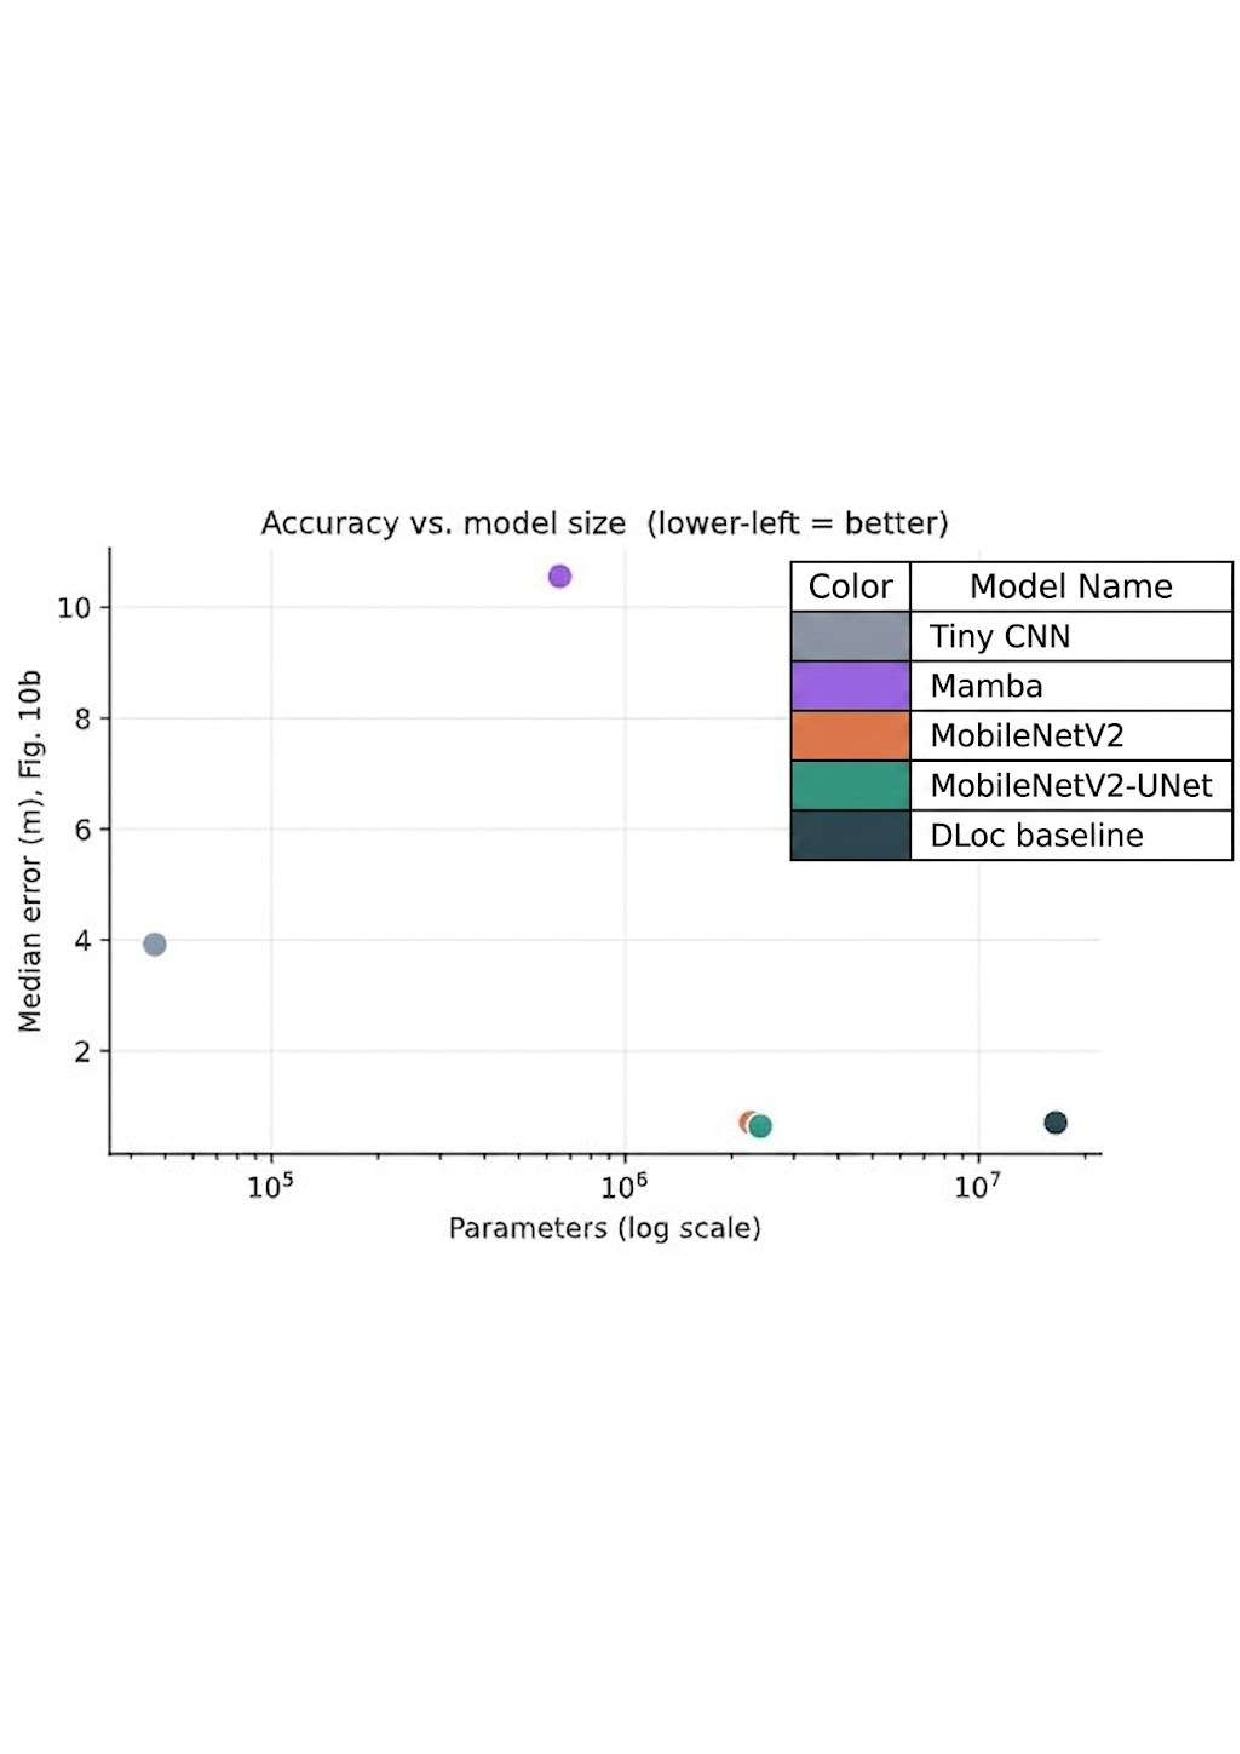
\includegraphics[width=0.66\linewidth]{compression_pareto}
\caption{Accuracy versus model size. The MobileNetV2-UNet sits at the favorable lower-left ---the best
median error of any model at a fraction of DLoc's parameters--- while Mamba (top) and TinyCNN mark the
two ways to fail: wrong framing and too little capacity.}
\label{fig:find:pareto}
\end{figure}

\section{Finding 3 --- Distillation buys robustness, not accuracy}
\label{sec:find:3}

\textbf{Claim.} In this heatmap task, knowledge distillation leaves clean accuracy unchanged but
sharply improves behavior under shift. \textbf{Evidence.} Standalone and distilled models share the
\emph{same} in-distribution median, yet distillation gives MobileNetV2 a $3.4\times$ better median
under $\sigma{=}0.1$ noise ($16.368\to4.769$\,m) and consistently helps on the hardest cross-session
fold. \textbf{Mechanism.} In distribution the teacher's soft heatmap is nearly identical to the ground
truth, so its term is redundant; off-distribution that ``spatial label smoothing'' regularizes the
student toward more tolerant features (Ch.~\ref{ch:distill}). \textbf{So what.} Distillation is worth
doing precisely for the realistic, degraded deployment case ---and judging it by clean accuracy alone
misses its entire value.

\section{Finding 4 --- Distillation has a capacity threshold ($\sim$2\,M)}
\label{sec:find:4}

\textbf{Claim.} Distillation helps only students above $\sim$2\,M parameters; below that it
\emph{hurts}. \textbf{Evidence.} It helps MobileNetV2 (2.3\,M) and MobileNetV2-UNet (2.41\,M) but
degrades TinyCNN (47\,K): under random 1-AP dropout TinyCNN worsens from 7.940 to 13.648\,m when
distilled. \textbf{Mechanism.} A tiny model has no spare capacity, so imitating the teacher's modeled
AP interactions crowds out its own fallback behavior; when an AP drops, those memorized interactions
become invalid. \textbf{So what.} Distillation is not free regularization ---it presupposes a student
rich enough to absorb the teacher's hints \emph{and} keep its own robustness.

\begin{keyidea}
Findings 3 and 4 together are the ``dual nature'' of distillation: the \emph{same} soft-target signal
\emph{regularizes} a large-enough student into robustness but \emph{overloads} a too-small one into
brittleness. One mechanism, two opposite outcomes, split at a capacity threshold.
\end{keyidea}

\section{Finding 5 --- The two robustness mechanisms are complementary, not additive}
\label{sec:find:5}

\textbf{Claim.} Skip connections and distillation each improve robustness, but against \emph{different}
corruptions, and stacking them does not simply add. \textbf{Evidence.} On the MobileNetV2-UNet, the
\emph{skips} dominate noise robustness (standalone $3.000$\,m at $\sigma{=}0.1$, a $5.5\times$ gain over
plain MobileNetV2), while \emph{distillation} dominates multi-AP dropout (random 2-AP:
$3.324\to2.730$\,m). Combining them under noise gives $3.469$\,m ---slightly \emph{worse} than the
standalone $3.000$, i.e.\ not additive. \textbf{Mechanism.} Skips provide an \emph{architectural} path
around a noisy bottleneck; distillation provides a \emph{training-time} feature regularizer. They
target different failure modes. \textbf{So what.} Choose the mechanism for the corruption you expect:
skips for high-noise environments, distillation for AP failures; do not assume both at once compounds.

\section{Finding 6 --- Cross-session accuracy is competitive for the cost}
\label{sec:find:6}

\textbf{Claim.} Under DLoc's own leave-one-session-out protocol, the compressed model is roughly on par
with published DLoc. \textbf{Evidence.} The MobileNetV2-UNet (3 seeds) reaches $0.852$, $0.822$,
$1.116$\,m on the three held-out August folds ---mean $0.930$\,m versus DLoc's $0.86$\,m. It
\emph{matches} DLoc on different-furniture ($0.822$ vs $0.82$), holds the \emph{same} average P90
($2.374$ vs $2.33$), and \emph{beats} DLoc's P90 on the reflector fold ($2.489$ vs $2.77$).
\textbf{Mechanism.} The skips generalize the spatial mapping well; the only soft spot is the reflector
median, where DLoc's consistency decoder helps most. \textbf{So what.} This is an honest
\emph{efficiency} result: near-DLoc generalization at $6.8\times$ fewer parameters, not a cross-session
accuracy win ---and the thesis states it that way.

\begin{figure}[H]
\centering
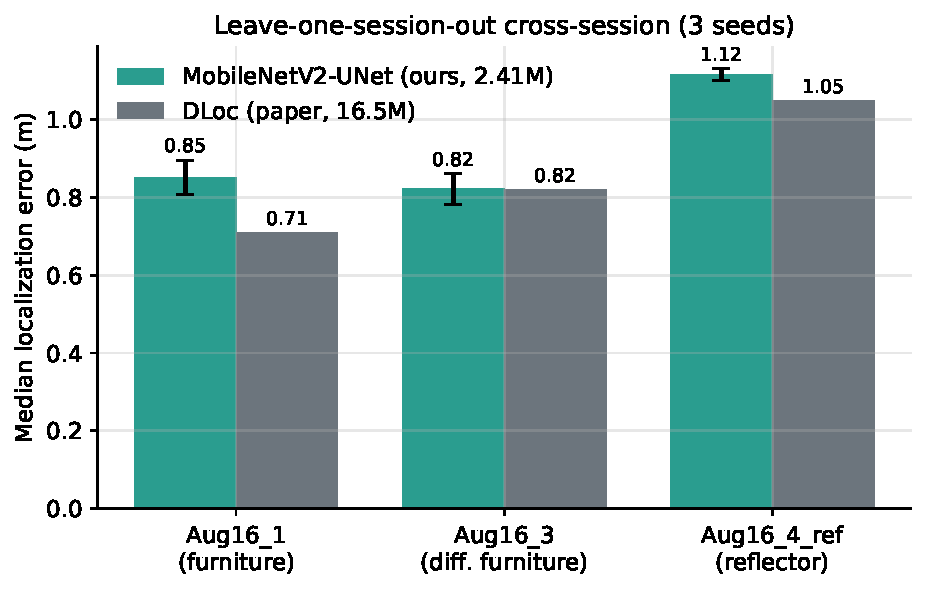
\includegraphics[width=0.7\linewidth]{crosssession_median}
\caption{Leave-one-session-out median error: our 2.41\,M MobileNetV2-UNet (three-seed mean $\pm$ std)
against the published 16.5\,M DLoc. The U-Net matches DLoc on the different-furniture fold and lands
within $\sim$0.1\,m on the others, at $6.8\times$ fewer parameters.}
\label{fig:find:crosssession}
\end{figure}

\begin{defensetip}
Frame Finding 6 carefully and you disarm the obvious challenge. Lead with ``competitive at $6.8\times$
compression,'' cite the fold it \emph{matches} and the P90 it \emph{beats}, and concede the small
reflector-median gap \emph{with its reason} (no consistency decoder). Honesty about the $\sim$0.07\,m
gap reads as rigor, not weakness.
\end{defensetip}

\section{The synthesis and the practical recommendation}
\label{sec:find:synthesis}

Put the six together and the thesis's answer to its own question ---``is DLoc's cost inherent?''--- is
a clear \emph{no}. A model an order of magnitude smaller can match or beat DLoc, provided you add the
right structure (skips) rather than parameters, and use distillation where capacity allows to harden
it against shift.

The practical recommendation that falls out:
\begin{itemize}[leftmargin=1.4em,nosep]
  \item \textbf{Default choice: distilled MobileNetV2-UNet.} Best in-distribution accuracy (0.640\,m),
  competitive cross-session, best under multi-AP dropout, and $56\times$ cheaper to run than DLoc.
  \item \textbf{If noise is the dominant threat:} the \emph{standalone} U-Net (its skips give the
  strongest noise robustness, which distillation slightly dilutes).
  \item \textbf{If raw compression is the only goal:} the distilled plain MobileNetV2 ---0.707\,m at
  just 2.3\,M parameters.
\end{itemize}
In every case, a model roughly an order of magnitude smaller than DLoc meets or exceeds its accuracy
---the single point the whole thesis is built to make.
